\chapter{Results}
\label{chapter3}

\section{Implementation}
The following section outlines the implementation steps taken to ensure the success of this project. This follows the method as described in the previous chapter, and details additional functionalities introduced to aid the main implementation steps.

\subsection{Data loaders}
The first implementation consideration was the project data loaders. Before we can start building solutions we require our dataset, so implementing the data loaders is a priority. The \code{loaders.py} file implements the functionality as overviewed below. As discussed earlier, the NWPU-RESISC45 dataset is readily available with a prebuilt data loader from \code{TensorFlow Datasets}, so all we require is a function that wraps the \code{TensorFlow Datasets} loading function, providing us with a single function to call whenever we wish to load the dataset. The remainder of the \code{loaders.py} file offers functionality for loading the Set5 and Set14 evaluation datasets, data loaders specifically for Linux-based file systems, and the function used to generate our stratified subset of the NWPU-RESISC45 dataset. The main goal of the \code{loaders.py} file is to provide a simple interface for the loading of our datasets where needed.

\subsection{Custom \code{Keras} components}
As explained in section~\ref{sec:tools_and_practices}, our implementation uses \code{Keras} to implement the neural network models. Good development practice with \code{Keras} involves creating custom components that can then be used in the exact same fashion as the native \code{Keras} components~\cite{keras}. In this project we implemented several custom \code{Keras} components to aid the solution development as a whole. The first of these was the custom \code{PixelShuffle} layer, which provides the functionality for upsampling the image during a forward pass of SRGAN.\@\code{Keras} did not provide the required functionality, so it was implemented by subclassing the \code{keras.Layer} class and overriding the call function so that it implemented the desired functionality. Alongside a custom layer, we also implemented two custom models to provide preprocessing and utility functionality. The first of these was the custom model \code{CropAndResize}, which is used to preprocess the HR ground truth images into the LR inputs used for model training. This model takes an image or set of images, selects a random $96 \times 96$ patch for each image, and then downsamples using bicubic interpolation with a downsampling factor of four, as described in the previous chapter. This implements the image patch generation mechanism. The second instance was the custom model \code{CustomLoss}, which was used to provide the forward pass through a pretrained classifier to retrieve the feature maps required for the perceptual loss component of SRGAN training. This custom loss model acted as a useful utility as it allowed us to pass the model to the class and then retrieve a model that produces the feature maps of an input image. Implementing these models by subclassing \code{Keras} classes is inline with good development practice and provides reusable classes and functions.

\subsection{SRResNet}
The implementation of SRResNet, the generator component of SRGAN, follows the same development practice as described in the previous section, but deserves its own overview due to the importance of the model in our solution. By subclassing the \code{keras.Model} interface we are able to customise many of the procedures involved with training SRResNet. The model architecture is implemented using native \code{keras.layers}. The functionality and structure of the layers themselves can be found in section~\ref{subsec:architecture}. Taking a variety of patches every update iteration requires us to customise the \code{train\_step} method, which decides how the model is trained on the input dataset. The \code{train\_step} function begins with the generation of the data for that iteration, where eight patches are taken from each of the 15 images in that batch. The patches are downsampled and then fed through SRResNet in its current state. The MSE is calculated between the generated image and the HR image to provide us with the total loss for that training iteration. Gradient descent in \code{Keras} is implemented using the \code{GradientTape} context to automatically calculate gradients. The calculated gradients were then used to update the gradients and step the model state towards producing a better SR reconstruction result. The \code{test\_step} function implements the calculation of the validation loss at each epoch end. This follows the exact same process as the \code{train\_step} function, however a validation dataset is used and the final MSE is used to measure the performance of the model after each training epoch, meaning the model weights are not changed.

\subsection{SRGAN}
SRGAN followed a very similar implementation procedure to SRResNet. The model implements the discriminator component using the \code{keras.layers} interface, and takes the pretrained generator from the SRResNet model itself. The train step takes image patches in the same way as the SRResNet \code{train\_step}, however the loss process is different. The generator and discriminator losses are calculated as described in the previous chapter, using the inbuilt binary cross-entopy loss and each of the custom losses. These losses are then used to update the generator and discriminator weights using gradient descent via \code{GradientTape}. The validation step is implemented the same as SRResNet, except the appropriate generator and discriminator losses are reported instead of the MSE loss.

\subsection{Custom losses}
The custom losses we create using the feature maps from pretrained classifiers can be found in the \code{losses.py} file. This file implements a class that contains a get method for every single custom loss we will use. Each of these get methods simply retrieves the pretrained classifier, strips the fully connected layers off the top, and instantiates the \code{CustomLoss} class described earlier to provide a model that calculates the feature maps for the image input. The \code{losses.py} file exists primarily to ensure reusable code and avoids redefining new loss functions within the training file. The result is a simple method for retrieving custom loss functions through a single method call.

\subsection{Training}
The \code{training.py} file organises the model training process due to the large number of models we need to train for this project. The file contains several functions, each designed to take arguments that decide how that particular model is trained. There is one function for SRResNet, and another for SRGAN.\@ The SRGAN model takes the \code{CustomLoss} class as an argument, which is then used as the perceptual loss component. The main reasoning for the \code{training.py} file is to create a simple interface for executing training. The model is implemented as a class, where calling the \code{train} method of that class with automatically begin training the model. The \code{train} method takes the model name and the number of epochs as arguments, and the class handles the rest of the setup and begins training. This enabled a more efficient workflow where we did not have to extensively edit code with every new model, but instead just passed two different arguments to a single method.

\subsection{Testing}
Testing model performance was implemented as a script in the \code{testing.py} file. We chose to use a simple script as the process only needs to execute once, as we can save the SSIM and PSNR model results. This file begins by loading the NWPU-RESISC45 test set, Set5, and Set14. Each of the saved models are then loaded. SR reconstructions of each of the LR evaluation set images are created, and the comparison between SR and HR is executed using SSIM and PSNR.\ The SSIM and PSNR methods are implemented using \code{scikit-image}, a \code{Python} library specialised in image processing. The final performance results for all models and all datasets are then saved into a CSV format.

\subsection{Utilities}
The final implementation details we offer are related to two utility functions, located in the \code{utils.py} file. Whilst not required for project success, they offer an interface to commonly used functions and keep the project inline with good development practices. The first of these is the \code{GANSaver} class, which saves the full model state after an epoch that has produced a validation loss lower than the current best. This class exists as the SRGAN model is composed of two models, which the inbuilt \code{Keras} model saver handled incorrectly. The second utility is the \code{visualise\_generator} function, which is used to visualise the SR reconstruction of a generator, primarily used whilst developing and training models to view how their outputs look. Overall these functions were incredibly useful during implementation and helped enforce good development practices by avoiding duplicating code.

\subsection{Justifying our implementation}
Each of the aforementioned implementation areas is designed to support the training, testing and evaluation of SRGAN, using the process explained and justified in Chapter 2. We use \code{Keras} for the implementation as described, meaning that every other implementation decision was made to best support the functionality of \code{Keras} and enforce good programming practices.

\section{Training}
The following section describes the steps taken to determine the parameters used for training and overviews the training durations.

\subsection{Parameter selection}\label{subsec:parameter_selection}
As explained in section~\ref{subsec:procedure}, we use a systematic approach to determine the training parameters, based on the memory constraints caused by our training hardware. We execute the following procedure.

The number of image classes in the NWPU-RESISC45 dataset is considered first. There are 45 distinct image classes, as listed in section~\ref{subsec:resisc45}. To avoid unintentionally overfitting our SR reconstruction model to a specific class we must include an equal number of images from each of the 45 classes, consequently requiring our dataset size to be a multiple of 45. Therefore, it is also required that the batch size factors into 45 to ensure that the entire dataset is visited over a single epoch and no training examples are skipped due to division remainders.

A larger batch size produces a smoother gradient and therefore more stable training, however the hardware available restricts how large the batch size can be~\cite{batchSizeTest}. Employing a method of trial and error identifies a batch size suitable for training the SR reconstruction model whilst adhering to memory constraints. A sample dataset of size 450 is used to test different batch sizes, with the intention of later increasing the dataset size to increase training examples. Firstly, training of the SRGAN model begins with a batch size and a single image patch per training example. The system attempts to allocate the required memory resources and computing power from the GPU but is unable to, resulting in an out-of-memory (OOM) exception. The batch size is then reduced, and the process is repeated until no OOM exception occurs. In practice the first batch size selected was $b = 30$, which resulted in an OOM exception. This value was reduced until a final batch size of $b = 15$ was selected. The next step was to test the memory constraints on the number of patches taken from each training example. A similar approach was taken to selecting batch size, where the number of patches was reduced until running model training no longer yielded an OOM exception. The initial value was $p = 16$, as suggested by Ledig et al., with the test yielding $p = 10$ patches per training instance. Further testing showed that for $p = 10$ and $p = 9$ that training would begin but that halt at seemingly random points in the process. To combat this, the number of patches was further reduced to $p = 8$, which yielded no OOM exceptions. Finally, the dataset size was selected by employing the same trial and error approach, where a dataset size of $n = 945$ was yielded. The final sizes are a batch size of $b = 15$, number of patches $p = 10$ and dataset size $n = 945$. Specific details on how the dataset subset was generated can be found in section~\ref{subsec:data_preparation}. We can also calculate the number of epochs and the number of steps per epoch (update iterations). An epoch step is defined as model training for one batch. Each image only appears once across all batches, meaning our total number of steps per epoch is:
\[\frac{\textnormal{Dataset size}}{\textnormal{Batch size}} = \frac{945}{15} = 63\]
Following the calculation of the steps per epoch, we are able to calculate the number of epochs required for $10^5$ and $10^4$ update iterations:
\[\Bigg\lceil\frac{10^5}{\textnormal{Steps per epoch}}\Bigg\rceil = \Bigg\lceil\frac{10^5}{63}\Bigg\rceil = 1588\]
\[\Bigg\lceil\frac{10^4}{\textnormal{Steps per epoch}}\Bigg\rceil = \Bigg\lceil\frac{10^4}{63}\Bigg\rceil = 159\]
The selection of batch size, dataset size and number of patches allows for remaining training details to be considered. As suggested by Ledig et al.\ the Adam optimiser is used with $\beta_1 = 0.9$, the SRResNet model is trained with a learning rate of $10^{-4}$, the initial training for the SRGAN model is trained with a learning rate of $10^{-4}$, and the fine-tuning training is executed with a learning rate of $10^{-5}$. The pretrained SRResNet model is used as the initial generator of the SRGAN model to reduce the likelihood of undesirable local optima~\cite{srgan}. The Ledig et al.\ procedure suggests $10^6$ update iterations for the pretrained SRResNet model. With the available training hardware and batch size, dataset size and number of patches training would take $\sim$48 hours. Due to the University of Leeds machines restarting every day, training the model for that long becomes tricky. As a result of this it makes sense to reduce the number of update iterations to $10^{5}$, reducing the training time to just over four hours. In interest of maintaining the guidance set out by Ledig et al.\ the number of update iterations for the first pass and fine-tune training of the SRGAN model should also be reduced by a factor of 10 to be proportional, yielding $10^4$ update iterations. Table~\ref{table:model_training} provides a summary of the training parameters for all training scenarios.
\begin{table}
    \centering
    \begin{tabular}{cccc}
        \toprule
        {} & \textbf{SRResNet} & \textbf{SRGAN 1\textsuperscript{st} pass} & \textbf{SRGAN 2\textsuperscript{nd} pass} \\
        \midrule
        \textbf{Batch size} & 15 & 15 & 15\\ 
        \textbf{Patches} & 8 & 8 & 8 \\
        \textbf{Dataset size} & 945 & 945 & 945\\
        \textbf{Adam $\beta_1$} & 0.9 & 0.9 & 0.9\\
        \textbf{Learning rate} & $10^{-4}$ & $10^{-4}$ & $10^{-5}$ \\
        \textbf{Update iterations} & $10^5$ & $10^4$ & $10^4$ \\
        \textbf{Epochs} & 1588 & 159 & 159 \\
        \textbf{Steps per epoch} & 63 & 63 & 63 \\
        \bottomrule
    \end{tabular}
    \caption{Summary of the details and parameters used for model training.}
    \label{table:model_training}
\end{table}

\subsection{Training duration}
It is worth mentioning the significant time invested towards training each of the solutions. Training SRResNet with MSE loss yielded $\sim$144ms per update iteration, giving a total training time of just over four hours. The training times of the SRGAN models varied based on the classifier used for the perceptual loss component. Deeper classifiers result in a forward propagation time, which is reflected in the time per update iteration. MobileNetV2 recorded the lowest time per update iteration at $\sim$400ms per update iteration, yielding a total training time of just over an hour. EfficientNetV2L produced the longest per update iteration at $\sim$750ms per update iteration, yielding a total time of just over two hours. These training times are for a single training pass, so fully training each SRGAN model takes twice as long. Taking the total training time across all models yields $\sim$35 hours. These calculations do not include the time spent training models during the development stage of the model, which far exceeds the aforementioned 35 hours.

\section{Performance results}
As discussed in section~\ref{sec:measuring_performance}, we use SSIM and PSNR to measure the performance of our final models. Model performance is calculated on three separate evaluation sets. First is the test set we have selected from the NWPU-RESISC45 dataset, which is stratified to include three images from each of the 45 classes, resulting in a total of 135 images. The other two testing sets are Set5 and Set14, widely used as evaluation sets in the field of SR reconstruction. The Set5 and Set14 datasets do not contain any remote sensing imagery. The purpose of calculating these performance metrics across with Set5 and Set14 is twofold. The first reason is to show that our solutions, trained on specifically remote sensing imagery, are better at creating SR reconstructions of remote sensing imagery. The second reason, albeit less important than the first, is for the test sets to act as additional comparators for individual model performance. The SSIM and PSNR metrics calculated on the aforementioned evaluation sets are showcased in table~\ref{fig:performance_results}.
\begin{table}
    \centering
    \begin{tabular}{ccccccc}
        \toprule
        {} & \textbf{SSIM} & {} & {} & \textbf{PSNR}  & {} & {} \\
        \midrule
        {} & \textbf{Test set} & \textbf{Set5} & \textbf{Set14} & \textbf{Test set} & \textbf{Set5} & \textbf{Set14} \\
        \midrule
        \textbf{Bicubic} & 0.9158 & \textbf{0.7824} & \textbf{0.6684} & 23.32 & \textbf{24.99} & \textbf{21.93} \\
        \textbf{SRResNet} & \textbf{0.9235} & 0.7643 & 0.6563 & \textbf{24.02} & 22.93 & 21.65 \\
        \textbf{SRGAN-VGG22} & 0.8994 & 0.5831 & 0.5131 & 23.05 & 21.53 & 20.84 \\
        \textbf{SRGAN-VGG54} & 0.8878 & 0.6686 & 0.6030 & 22.85 & 22.18 & 21.76 \\ 
        \textbf{SRGAN-Xception} & 0.8935 & 0.6722 & 0.6018 & 23.13 & 21.28 & 21.01 \\  
        \textbf{SRGAN-ResNet152V2} & 0.8916 & 0.6613 & 0.6021 & 22.90 & 22.09 & 21.83 \\ 
        \textbf{SRGAN-InceptionV3} & 0.8973 & 0.6860 & 0.6164 & 23.27 & 21.52 & 21.29 \\ 
        \textbf{SRGAN-InceptionResNetV2} & 0.9018 & 0.6824 & 0.6103 & 23.39 & 22.2 & 21.61 \\ 
        \textbf{SRGAN-MobileNetV2} & 0.8928 & 0.6925 & 0.6169 & 21.78 & 20.61 & 20.39 \\ 
        \textbf{SRGAN-DenseNet201} & 0.9045 & 0.6978 & 0.6299 & 23.47 & 21.63 & 21.79 \\
        \textbf{SRGAN-NASNetLarge} & 0.8930 & 0.6637 & 0.5966 & 23.03 & 20.86 & 20.96 \\
        \textbf{SRGAN-EfficientNetV2L} & 0.8958 & 0.5750 & 0.5263 & 22.54 & 19.65 & 20.01 \\
        \bottomrule
    \end{tabular}
    \caption{SSIM and PSNR results calculated on the test subset of NWPU-RESISC45, Set5, and Set14.}
    \label{fig:performance_results}
\end{table}
Calculating our performance metrics for each of the trained SRGAN models enables us to refer back to the conjecture presented in section~\ref{subsec:improving_loss}: `using the feature maps from more accurate image classification models in the perceptual loss component of SRGAN-based models will increase SR reconstruction performance'. We have the accuracy metrics for each of the pretrained classifiers, and we now how the SR reconstruction capabilities of each of the models, measured with SSIM and PSNR.\@ Therefore, we can review how these performance metrics change as the classifier accuracy increases. Plotting the Top-1 accuracy against SSIM and PSNR achieves this goal, with a line of best fit acting as a trend line. Figure~\ref{fig:performance_metric_vs_classifier_accuracy} shows the outcome of this simple test.
\begin{figure}
    \centering
    \begin{minipage}{0.5\textwidth}
        \centering
        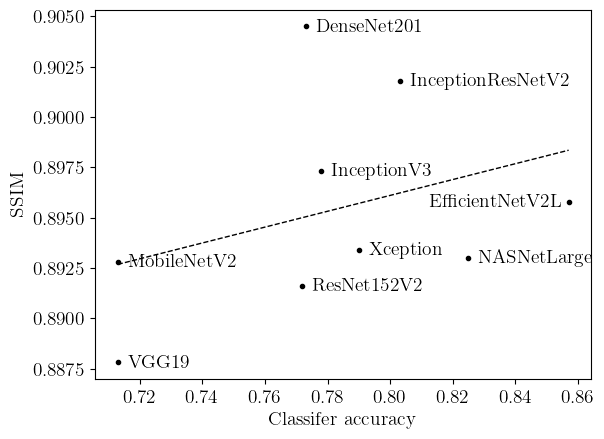
\includegraphics[width=\textwidth]{./assets/ssim_accuracy_trend.png} % first figure itself
    \end{minipage}\hfill
    \begin{minipage}{0.5\textwidth}
        \centering
        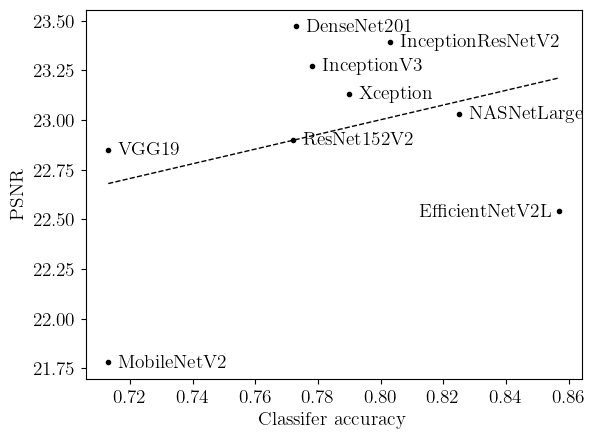
\includegraphics[width=\textwidth]{./assets/psnr_accuracy_trend.png} % second figure itself
    \end{minipage}
    \caption{Two scatter plots showing how the performance metrics of SRGAN models changed based on the accuracy of the classifer used for the perceptual loss component.}
    \label{fig:performance_metric_vs_classifier_accuracy}
\end{figure}

\section{Findings}
The following section overviews the findings following our implementation of the proposed solutions. We evaluate these findings in the next chapter.
\begin{itemize}
    \item \textbf{Individual model performance:} SRGAN-DenseNet201 performed the best out of the SRGAN models for both SSIM and PSNR. SRResNet performed better than all SRGAN models for both SSIM and PSNR. Bicbuic interpolation performed better than all SRGAN variants for both SSIM and PSNR, but failed to beat SRResNet.
    \item \textbf{Remote sensing specialisation:} SRResNet and all SRGAN variants performed better on remote sensing datasets compared to the Set5 and Set14 datasets, especially for SSIM.
    \item \textbf{Improving loss:} SRGAN-DenseNet201 outperforms SRGAN-VGG54 (the model proposed by Ledig \etal), showing that we are able to produce better SR reconstruction results with SRGAN by using the feature maps from a more accurate classifier as the perceptual loss component.
    \item \textbf{Addressing our conjecture:} Comparing classifier accuracy and reconstruction capabilities in figure~\ref{fig:performance_metric_vs_classifier_accuracy} suggests that there is a positive relationship between classification accuracy and SR reconstruction capabilities when utilised as a perceptual loss component.
    \item \textbf{Visual quality and MOS:} Manually reviewing reconstructions suggest that SSIM and PSNR may not accurately reflect human perception of quality. SRResNet, which achieves the highest SSIM and PSNR for the remote sensing dataset appears overly blurred, and SRGAN-VGG54 appears to produce the results with the closest similarity to the HR ground truth.
    \item \textbf{Noise and artefacts:} In several of the models, especially SRGAN-EfficientNetV2L, -MobileNetV2, and -VGG22 we can see clearly visible artefacts in the form of irregular pixel values. We can also see interesting grid like noise patterns in some reconstructions.
\end{itemize}



